
%%% Local Variables:
%%% mode: latex
%%% TeX-master: t
%%% End:

\chapter{正例去噪算法研究}
\label{cha:2}
对于个性化推荐应用而言,最广泛使用的隐式反馈是一种不完全数据(incomplete data),只能观察到交互的有无,而无法观察到该交互所对应偏好的大小。隐式反馈数据中通常包含一些不可信交互(误报),即伪正例,例如代购、误触等交互数据。由这些伪正例构建的成对比较,是不可信的成对比较,也称为含噪声成对比较,导致成对学习模型的不准确优化。本章提出一种自适应去噪的成对排序算法(Bayesian Personalized Ranking with Autonomous Credence, BPRAC),用于从含噪成对比较的数据中学习个性化排序。由于交互对应的偏好值不可观测,本章引入一个隐变量作为衡量交互置信度的新指标,这个隐变量与用户物品表示一起作为模型参数进行端到端地学习。所提出的BPRAC算法采用期望最大化框架:在期望步骤中使用贝叶斯推断来估计交互的置信度指标;在最大化步骤中固定置信度指标,更新参数学习用户和物品的表示。在真实世界的数据集上进行的实验证实自适应去噪的成对排序算法的优越性。

\section{引言}
噪声的存在会对机器学习模型的性能和泛化能力产生负面影响。首先,噪声可能导致模型对数据的过拟合。模型可能会将噪声视为真实模式,从而导致错误的学习和预测。其次,噪声可能降低模型的准确性和稳定性。如果训练数据包含大量噪声,模型可能无法准确地捕捉数据的真实分布和模式,从而导致预测结果的不可靠性。噪声在机器学习中广泛存在,可以来自多个方面,包括数据收集过程中的错误、不准确的标注、不完整的数据、异常值等。隐式反馈数据是典型的不完全数据,只能观测到用户的交互记录,但是无法观测到交互所对应偏好的高低。隐式反馈数据中存在一些用户的手滑、误触、代购等无偏好的交互行为,会被记录并当作正例,构成了伪正例问题。

如图~\ref{Fig2-1}所示,一个运动爱好者在节日期间给女友购买了一个口红$i_3$,这是一个不体现该用户偏好的偶然交互行为。成对比较是由已经交互的正例和未交互的负例构成,由于$i_3$是伪正例,任何包含$i_3$的成对比较,都是噪声成对比较。如果不能消除这些噪声成对比较的影响,推荐模型会误认为该运动爱好者更偏好口红而非其他运动物品,从而产生一系列例如女性用品的错误推荐结果。
\begin{figure}[!htbp]
	\centering
	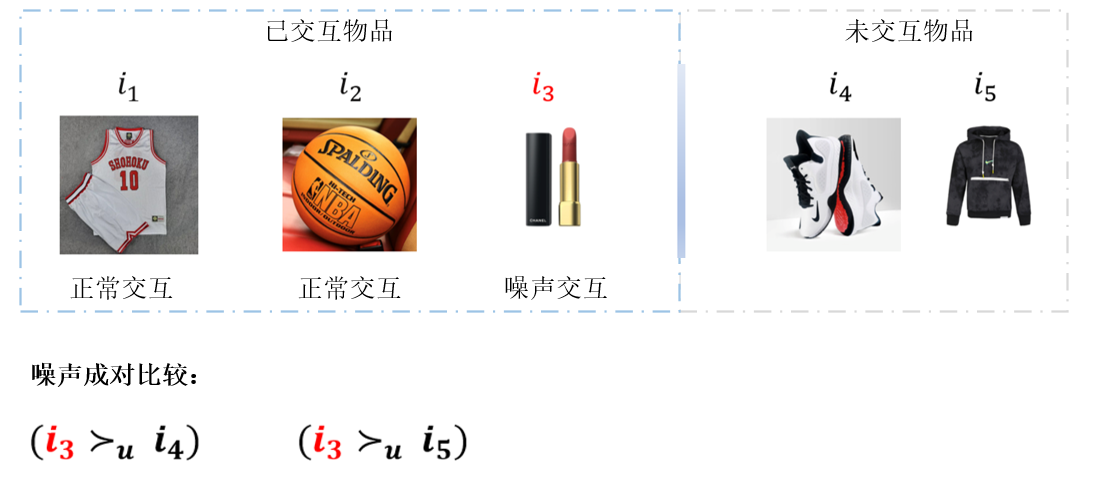
\includegraphics[scale=0.3]{2-IllustrativeExample.png}
	\caption{含噪成对比较示意图}
	\label{Fig2-1}
\end{figure}

一般而言,存在两种类型的噪声:一种是特征依赖的噪声\cite{Menon:2018:ML},例如标注者可能倾向于混淆狼和狗,但不会混淆老虎和狗,因此狼容易被错误标注而老虎不会;另外一种是独立于特征的噪声\cite{patrini:2017:CVPR},如高斯白噪声。推荐系统的误报兼具二者特征。例如误触,与物品的特征无关,每个交互的噪声率是随机均匀分布的;而代购,则与物品的特征有关,具有礼物性质的物品更容易产生较高的噪声率。

在机器学习的基础理论方面,先前的研究解决标签噪声学习主要是从数据、目标函数和优化策略的角度出发,并提出了相应的解决方法和技术。具体而言,从数据的角度,重点是建立并估计噪声转移矩阵,该噪声转移矩阵模拟了标签错误的过程,可以用于还原数据的原始的所属类别~\cite{Van:2017:JMLR}。这个噪声转移矩阵还可以用来校正损失,构建与干净数据风险一致的估计\cite{xia:2019:NIPS}。从目标函数的角度出发,主要思路是经验风险重写(Empirical Risk Rewriting)。例如文献~\cite{liu2015classification}通过重加权样本设计能够容忍噪声的损失函数,它可以比标准损失函数更具鲁棒性。最后,从优化策略的角度出发,重点是探索优化的动态过程,以解决标签噪声学习问题。核心在于,神经网络倾向于先拟合干净数据,然后拟合噪声数据\cite{zhang2021understanding}。基于这一发现,例如早停法~\cite{li2020gradient}作为一种简单而有效的方法,用于避免在噪声数据上过拟合;而Co-teaching方法~\cite{Han:2018:NIPS}通过小损失技巧相互筛选干净样本,鲁棒地同时训练两个网络。

在成对学习的问题设置下,噪声问题更具挑战性。例如从优化策略出发的“神经网络倾向于先拟合干净数据,然后拟合噪声数据”的经验性观察主要是基于单个样本构建的损失,是否在成对样本构建的损失上依旧起作用是存疑的,因为在推荐中往往是难以拟合的困难样本对性能的提升贡献越大\cite{Steffen:2014:WSDM}。此外,由于推荐系统中的噪声既具有特征依赖性又具有特征无关性,使用噪声转移矩阵模拟噪声标签的生成过程或估计权重以对样本进行重加权都变得非常具有挑战性。回溯伪正例的本质,是隐式反馈数据的特性造成的
:它是一种不完全数据,无法观测到交互所对应的偏好值,才产生了噪声成对比较。如果能观测到每个交互偏好强度的高低,那么根据偏好值大小值构造的成对比较就是可靠的。从统计视角,期望-最大化(Expectation-Maximazation)最大化框架是一个从不完全数据中进行极大似然或者最大后验估计非常有效的方法,可以估计无法观测到的隐变量和模型参数。因此,本章引入一个隐变量,含义为每个交互的偏好值,同时也对应了每个成对比较置信度的高低,交互的偏好值越大则成对比较的置信度越高。从噪声成对比较中学习排序则转化为一个含有隐变量的最大后验估计问题:在期望步骤中使用贝叶斯推断来估计置信度指标;在最大化步骤中固定置信度指标,更新模型参数学习用户和物品的表示,以减少噪声成对比较对学习算法的影响,学习更加准确的用户和物品表示。

\section{自适应去噪的成对排序算法}
\subsection{问题设置}
设$\mathbf{X}=[x_{ui}] \in \mathbb{R}^{M\times N}$表示包含$M$个用户和$N$个物品的交互矩阵,其中$x_{ui}\in \{1,0\}$。令$\mathcal{U}$和$\mathcal{I}$分别表示用户集合和物品集合。对于用户$u \in \mathcal{U}$,令$\mathcal{I}_u^+ \subseteq \mathcal{I}$表示他交互过的物品集合,$\mathcal{I}_u^- = \mathcal{I}\backslash \mathcal{I}_u^+$表示他未交互过的物品集合。通过选择一个属于$\mathcal{I}_u^+$的物品$i$和一个属于$\mathcal{I}_u^-$的物品$j$,可以构建成对比较的实例。训练数据集可以通过以下方式构建:
\begin{equation}\label{Eq2:obj}
	\mathcal{D} =  \left\{ {(u,i,j)|i \in \mathcal{I}_u^ +  \wedge j \in \mathcal{I}_u^ - } \right\}.
\end{equation}

BPR的目标是从训练数据集中学习用户和物品表示$\Theta$,使得观测到$\mathcal{D}$的后验概率最大化,即:
\begin{equation}\label{Eq:BPRObjective}
\mathcal{L}_\textsc{BPR} = \prod_{(u,i,j) \in \mathcal{D}} P(i \succ_u j|\Theta)P(\Theta).
\end{equation}
如果一个交互$x_{ui}=1$是噪声(伪证里),则所有包含$i$的成对比较$i \succ_u j$即为噪声比较,它们描述了不准确的用户偏好结构。这些噪声成对比较不应该包含在最大后验目标之内,否则会学到不准确的用户物品表示。然而,由于无法观测哪些交互是可信的,因此引入新的参数$c_{ui}$作为隐变量来衡量成对比较$i \succ_u j$的置信度。具体而言,对于一个可信的交互,$c_{ui}=1$;否则,$c_{ui}=0$。那么可以修正BPR的优化目标为:
\begin{equation}\label{Eq:Objective}
\mathcal{L}\prime = \prod_{(u,i,j) \in \mathcal{D}} [P(i \succ_u j|\Theta)P(\Theta)]^{c_{ui}}.
\end{equation}
其中,$c_{ui}$是隐藏变量,对交互项$(u,i)$进行加权。当$c_{ui} \rightarrow 0$(即不可信的交互)时,噪声比较$i \succ_u j$的后验概率被固定为1,用户和物品表示$\Theta$的更新不受该噪声成对比较的影响。作为一个可学习的变量,隐变量$c_{ui}$提供了从噪声数据中进行表示学习的解决方案。从含噪成对比较中学习排序的问题,可以形式化为一个含有隐变量的最大后验估计问题。

跟随BPR论文的符号规则,使用$\hat{x}_{ui}$来表示用户$u$对物品$i$的偏好预测值。用户偏好物品$i$胜过物品$j$的似然为:
\begin{equation}\label{Eq2:Sigma}
	P(i \succ_u j | \Theta) = \sigma(\hat{x}_{ui} - \hat{x}_{uj}),
\end{equation}
其中,$\sigma(\cdot)$是Sigmoid函数:$\sigma(z) = \frac{1}{1+e^{-z}}$。将公式\eqref{Eq2:Sigma}带入公式\eqref{Eq:Objective}中,并两边取对数,得到了如下最终的优化目标:
\begin{equation}\label{Eq:LogObjective}
\ln	\mathcal{L}\prime = \sum_{(u,i,j) \in \mathcal{D}} c_{ui}\left[\ln \sigma(\hat{x}_{ui} - \hat{x}_{uj}) - \lambda \|\Theta\|^2 \right],
\end{equation}
其中,$\lambda \|\Theta\|^2$是模型训练中的正则化项。下面介绍在矩阵分解模型下,如何求解这个含有隐变量的最大后验估计问题。
\subsection{先验分布}
BPR论文设定了用户物品表示为两个$d$维高斯随机向量的内积,基于矩阵分解得到的相似度分数先验分布由如下引理给出。
\begin{lemma}\label{Lemma2:AprioriDistribution}
设$x=\langle \mathbf{w}, \mathbf{h} \rangle$表示两个$d$维随机向量的内积,其中$\mathbf{w}$和$\mathbf{h}$的元素是独立同分布的随机变量,每个随机变量都服从$\mathcal{N}(0, \lambda)$的高斯分布。那么$x$的概率密度函数(PDF)为:
	\begin{equation}
		f_{X}(x; d, \lambda) = \frac{1}{\lambda \sqrt{\pi} \Gamma(\frac{d}{2})}\left(\frac{|x|}{2\lambda} \right)^{\frac{d-1}{2}}K_{\frac{d-1}{2}}\left(\frac{|x|}{\lambda}\right),
	\end{equation}
	其中,$K_{\eta}(\cdot)$是第三类修正的贝塞尔函数,$\Gamma(\cdot)$是伽玛函数。
\end{lemma}
\begin{proof}
随机变量$x=\langle \mathbf{w}, \mathbf{h} \rangle$可以通过以下代数运算转化为两个伽玛分布的随机变量的差:
\begin{eqnarray}
	x &=& \langle {\mathbf{w}},{\mathbf{h}} \rangle = \sum\nolimits_{k = 1}^d {w_k} \cdot {h_{k}} \nonumber\\
	&=& \frac{{{\lambda }}}{2}\sum\nolimits_{k = 1}^d {[\frac{{{{({w_{k}} + {h_{k}})}^2}}}{{2{\lambda  }}} - } \frac{{{{({w_{k}} - {h_{k}})}^2}}}{{2{\lambda  }}}]
\end{eqnarray}
那么
\begin{equation}
	\frac{2}{{{\lambda  }}}x = \sum_{k = 1}^{d} \frac{{{{({w_{k}} + {h_{k}})}^2}}}{{2{\lambda }}} - \sum_{k = 1}^{d} \frac{{{{({w_{k}} - {h_{k}})}^2}}}{{2{\lambda  }}},
\end{equation}
其中 $\frac{(w_k + h_k)}{\sqrt {2{\lambda}}} \sim \mathcal{N}(0,1)$, $\frac{(w_k - h_k)}{\sqrt {2{\lambda}}} \sim \mathcal{N}(0,1)$. 于是第一项${z_1} = \sum\nolimits_{k = 1}^d {\frac{{{{({w_{k}} + {h_{k}})}^2}}}{{2{\lambda }}}} $ 和第二项 ${z_2} = \sum\nolimits_{k = 1}^d {\frac{{{{({w_{k}} - {h_{k}})}^2}}}{{2{\lambda }}}} $ 服从自由度为$d$的卡方分布。 注意到卡方分布${\chi ^2}(d)$ 是参数为$Ga(z;\frac{d}{2},\frac{1}{2})$的伽玛分布族的特例, 因此变量${Z_1}$ and $ - {Z_2}$ 的特征函数为:
%a3
\begin{eqnarray}
	{\phi _{{Z_1}}}(t) &=& {(1 - 2it)^{ - \frac{d}{2}}}, \\
	{\phi _{ - {Z_2}}}(t) &=& {(1 + 2it)^{ - \frac{d}{2}}},
\end{eqnarray}
其中 $i$ 为虚数单位。 进一步地,记随机变量 $Y = \frac{2}{{{\lambda }}}X  = {Z_1} + ( - {Z_2})$, 则随机变量Y的特征函数 ${\phi _Y}(t)$是${\phi _{{Z_1}}}(t)$ 和 ${\phi _{ - {Z_2}}}(t)$的乘积:
\begin{equation}
	{\phi _Y}(t) = {\phi _{{Z_1}}}(t) \cdot {\phi _{ - {Z_2}}}(t) = {(1 + 4{t^2})^{ - \frac{d}{2}}}.
\end{equation}
那么随机变量Y的概率密度函数${f_Y}(y)$可以通过如下傅里叶逆变换计算得到:
\begin{equation}
	\begin{split}
		{f_Y}(y) &= \frac{1}{{2\pi }}\int_{ - \infty }^\infty  {{\phi _Y}(t){e^{ity}}dt} \\
		& = \frac{1}{{2\pi }}\int_{ - \infty }^\infty  {{{(1 + 4{t^2})}^{ - \frac{d}{2}}}{e^{ity}}dt}.
	\end{split}
\end{equation}

\par
直接计算上式${f_Y}(y)$是复杂的。观察到特征函数${\phi_Y}(t)$与方差伽玛(VG)分布~\cite{Madan:1990:Business,Senata:2004:ApplyPro}的特征函数具有相同的函数形式。VG分布的特征函数为
\begin{equation}
	{\phi _{VG}}(t) = E({e^{itX}}) = {e^{i\delta t}}{(1 - i\theta vt + \frac{{{\sigma ^2}v}}{2}{t^2})^{ - {1 \mathord{\left/
					{\vphantom {1 v}} \right.
					\kern-\nulldelimiterspace} v}}}.
\end{equation}
VG分布的概率密度函数${f_{VG}}(y)$为:
\begin{equation}
	\begin{aligned}
		{f_{VG}}(y;\theta ,\delta ,\sigma ,v) = \frac{{2e\frac{{\theta (y - \delta )}}{{{\sigma ^2}}}}}{{\sigma \sqrt {2\pi } {v^{\frac{1}{v}}}\Gamma (\frac{1}{v})}}{(\frac{{|y - \delta |}}{{\sqrt {\frac{{2{\sigma ^2}}}{v} + {\theta ^2}} }})^{\frac{1}{v} - \frac{1}{2}}}
		\cdot {{\rm K}_{\frac{1}{v} - \frac{1}{2}}}(\frac{{|y - \delta |\sqrt {\frac{{2{\sigma ^2}}}{v} + \theta } }}{{{\sigma ^2}}}).
	\end{aligned}
\end{equation}
取$\delta$=0, $\theta $=0, $v$=2/d, $\sigma$=$2\sqrt d$,那么
\begin{equation}
	{\phi _{VG}}(t) = {(1 + \frac{1}{4}{t^2})^{ - \frac{d}{2}}} = {\phi _Y}(t),
\end{equation}
由于特征函数与概率密度函数是一一对应的关系,因此Y的概率密度函数为
\begin{equation}
	\begin{split}
		{f_Y}(y) &= {f_{VG}}(y;\theta  = 0,\delta  = 0,\sigma  = 2\sqrt d ,v = \frac{2}{d})\\
		& = \frac{1}{{\sqrt {2\pi d} {{\left( {\frac{2}{d}} \right)}^{\frac{d}{2}}}\Gamma (\frac{d}{2})}}{(\frac{{|y|}}{{2d}})^{\frac{{d - 1}}{2}}}{{\rm K}_{\frac{{d - 1}}{2}}}(\frac{{|y|}}{2})\\
		& = \frac{1}{{\sqrt {2\pi } {2^{\frac{d}{2}}}\Gamma (\frac{d}{2})}}{(\frac{{|y|}}{2})^{\frac{{d - 1}}{2}}}{{\rm K}_{\frac{{d - 1}}{2}}}(\frac{{|y|}}{2}).
	\end{split}
\end{equation}

\par
需要注意的是,$\frac{{{\lambda }}}{2}Y = X$。通过将$Y$按照常数$\rho$进行缩放,可以生成一个经过缩放的随机变量分布
\begin{equation}
	\rho Y \sim \frac{1}{\rho }{f_Y}(\frac{y}{\rho }).
\end{equation}
取 $\rho  = \frac{{{\lambda  }}}{2}$,则$X = \frac{{{\lambda }}}{2}Y \sim \frac{2}{{{\lambda }}}{f_Y}(\frac{2}{{{\lambda }}}y)$,进而可以得到随机变量$X$的概率密度函数为:
\begin{equation}
	f_{X}(x; d, \lambda) = \frac{1}{\lambda \sqrt{\pi} \Gamma(\frac{d}{2})}\left(\frac{|x|}{2\lambda} \right)^{\frac{d-1}{2}}K_{\frac{d-1}{2}}\left(\frac{|x|}{\lambda}\right),
\end{equation}
\end{proof}
在BPR中,论文假设参数用户和物品的表示$\Theta$服从零均值和对角协方差矩阵的多元高斯分布,那么参数矩阵$\Theta$的所有元素都是独立且同分布(i.i.d)的随机变量,每个随机变量都服从$\mathcal{N}(0, \lambda)$的高斯分布。按照如上的多元高斯分布初始化后,使用引理\ref{Lemma2:AprioriDistribution}的结果,可以得到基于矩阵分解的偏好预测值的分布为:
\begin{equation}\label{Eq:PDFInnerProduct}
	f(\hat{x}_{ui}) = \frac{1}{\lambda \sqrt{\pi} \Gamma(\frac{d}{2})}\left(\frac{|\hat{x}_{ui}|}{2\lambda} \right)^{\frac{d-1}{2}}K_{\frac{d-1}{2}}\left(\frac{|\hat{x}_{ui}|}{\lambda}\right),
\end{equation}
相应的累积分布函数(CDF)为:
\begin{equation}\label{Eq:CDFInnerProduct}
	F(\hat{x}_{ui}) = \int_{-\infty}^{\hat{x}_{ui}} f(t)d(t).
\end{equation}

\subsection{后验分布}\label{Sec:Posterior}
考虑$n$个独立同分布的随机变量$\{Z_i\}_{i=1}^n$,其对应的取值$\{z_i\}_{i=1}^n$按升序排列:$X_1 \le X_2 \le \cdots X_n$,其中$X_k$是取值$x_k$在第$k$个位置的随机变量,那么$x_k$的概率密度为
\begin{equation}\label{Eq:PosteriorPDF}
	\begin{aligned}
		g({x_k};k,n)
		=   \frac{{n!}}{{(k - 1)!(n - k)!}} {[\Phi({x_k})]^{k - 1}}\phi({x_k}){[1 - \Phi({x_k})]^{n - k}}.
	\end{aligned}
\end{equation}
对于一个交互,只存在两种可能:(1)它是真正例,即用户真的喜欢;(2)它是伪正例,即用户不喜欢。预测评分只存在两个总体,于是取$n=2$。此外,模型是针对负例评分小于正例评分优化,对于关心的真正例的预测评分$\hat{x}_{ui}$,如果它是用户喜欢的正例,应该满足$\hat{x}_{uj}\leq \hat{x}_{ui}$,这正是次序统计量$X_{(2)}$的取值。于是可以写出真正例的预测评分$\hat{x}_{ui}$的分布
\begin{eqnarray}\label{Eq:ConditionalDistribution}
	g(\hat{x}_{ui};k=2,n=2)
	& = & \frac{2!}{(2-1)!(2-2)!}[F(\hat{x}_{ui})]^{2-1} f(\hat{x}_{ui}) [1 - F(\hat{x}_{ui})]^{2-2} \nonumber \\
	& = & 2 F(\hat{x}_{ui})f(\hat{x}_{ui}),
\end{eqnarray}
其中 $f(\cdot)$由公式\ref{Eq:PDFInnerProduct}给出,$F(\cdot)$由公式\ref{Eq:CDFInnerProduct}给出。图\ref{Fig:Prior}绘制了不同参数下先验分布示意图,图\ref{Fig:Posterior}绘制了不同参数下后验分布示意图,可以看到先验分布和后验分布满足非负性和归一性条件。
\begin{figure*}[t]
	\centering
	\subfloat{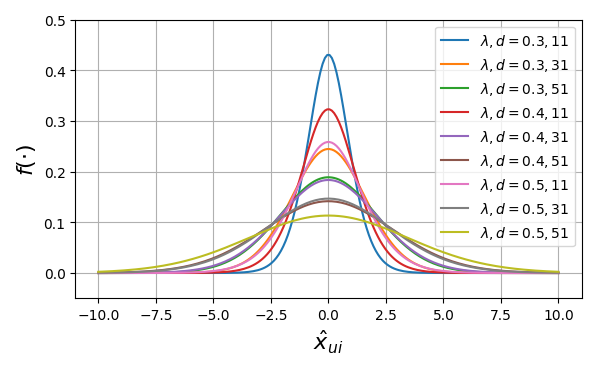
\includegraphics[width=.5\textwidth]{2-PriorPDF.png}}
	\subfloat{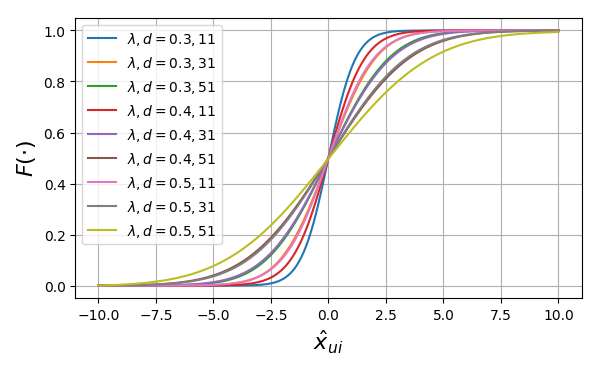
\includegraphics[width=.5\textwidth]{2-PriorCDF.png}}
	\caption{不同参数下先验分布示意图}
	\label{Fig:Prior}
\end{figure*}

\begin{figure*}[t]
	\centering
	\subfloat{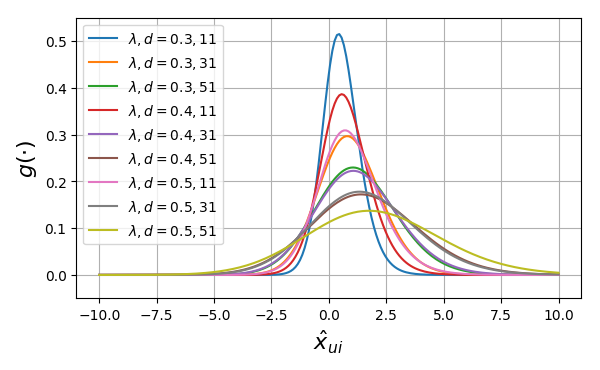
\includegraphics[width=.5\textwidth]{2-PosteriorPDF.png}}
	\subfloat{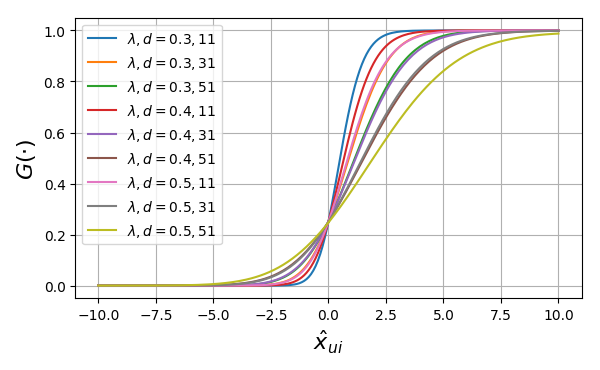
\includegraphics[width=.5\textwidth]{2-PosteriorCDF.png}}
	\caption{不同参数下后验分布示意图}
	\label{Fig:Posterior}
\end{figure*}

\subsection{学习算法}
在本节中,介绍了的学习算法并分析了其收敛性。该学习算法在EM框架下包括两个步骤:(i) 在期望步骤中估计$c_{ui}$,以及(ii) 在最大化步骤中学习用户和物品表示$\Theta$。

\subsubsection{期望步骤}
在期望步骤中,固定的模型参数$\Theta$,即给定预测评分,目标是估计$c_{ui}$。首先写出$Q(\cdot)$函数为 
\begin{eqnarray}\label{Eq:QDef}
 Q(\Theta, \Theta^{(t)}) 
	& = & \mathbb{E}_{c_{ui} } \left[ \ln P(\Theta|\succ_u, c_{ui}) | \succ_u, \Theta^{(t)} \right] \nonumber \\
	& = & \mathbb{E}_{c_{ui}} \left[ \Sigma_{(u,i,j)\in \mathcal{D}} c_{ui} \left( \ln \sigma(\hat{x}_{ui} - \hat{x}_{uj}) - \lambda \| \Theta \|^2 \right) \right] \nonumber \\
	& = & \Sigma_{(u,i,j) \in \mathcal{D}} \mathbb{E}[c_{ui}] \left[ \ln \sigma(\hat{x}_{ui} - \hat{x}_{uj}) - \lambda \| \Theta \|^2 \right],
\end{eqnarray}
其中,$\mathbb{E}[c_{ui}]$是给定在第$t$次学习迭代中模型参数$\Theta^{(t)}$的条件下,$c_{ui}$的期望值。使用$\mathbb{E}[c_{ui}]$作为$c_{ui}$的估计。由于$c_{ui}$是一个二值伯努利变量,有以下关系式:
\begin{eqnarray}
 \hat{c}_{ui}=	\mathbb{E}[c_{ui}] &=& P({c_{ui}} = 1|\Theta,{ \succ _u}) \nonumber \\
	&=& P({c_{ui}} = 1|{\hat{x}_{ui}} ,\succ_u)  \label{Eq:EStimationCui} \\
	&=& \frac{ P( {\hat{x}_{ui}},{ \succ_u}|{c_{ui}} = 1)}{ P({\hat{x}_{ui}} ,\succ_u)}{P({c_{ui}} = 1)} \label{Eq:Bayes}\\
	&\propto& P( {\hat{x}_{ui}},{ \succ_u}|{c_{ui}} = 1)P({c_{ui}} = 1) \label{Eq:Bayesian} \\
	&=& g({{\hat x}_{ui};n=2,k=2})P({c_{ui}} = 1) \label{Eq:ClassDensity}
\end{eqnarray}
需要注意的是,当固定模型参数$\Theta$时,预测评分$\hat{x}_{ui}$也被固定,于是有公式\eqref{Eq:EStimationCui}。公式\eqref{Eq:Bayes}是基于贝叶斯公式得到,其中$P(c_{ui}=1)$是交互为可信的先验概率,分母$P(\hat{x}_{ui},\succ_u)$在贝叶斯分析中被省略为归一化常数。$P(\hat{x}_{ui},\succ_u|c_{ui}=1)$是可信交互的概率密度。给定所有的预测评分,对于一个可信的交互$(u,i)$,其预测评分$\hat{x}_{ui}$应该满足$\hat{x}_{uj} \leq \hat{x}_{ui}$,此时概率密度由公式\eqref{Eq:ConditionalDistribution}给出。在给定$P(c_{ui}=1)$的情况下,观测值$\hat{x}_{ui}$在分布$g({{\hat x}_{ui};n=2,k=2})$中对应的概率密度越高,它是可信交互的可能性越大。

设$n_i$表示物品$i$的选择比例,即与该物品进行交互的用户的百分比。令$\bar{n}$和$\sigma_n$分别表示交互比例的平均值和标准差。通过以下方式计算$P(c_{ui} =1)$:
\begin{eqnarray}
	P(c_{ui} =1) = \mathsf{sigmoid}(\frac{n_i - \bar{n} }{\sigma_n}).
\end{eqnarray}
其中$\mathsf{sigmoid}$函数的作用是将输入转换为$(0,1)$范围内的概率。
\subsection{最大化步骤}
在最大化步骤中,固定隐变量$\hat{c}_{ui}$, 然后学习模型参数$\Theta$以最大化$Q(\cdot)$函数,即
\begin{equation}\label{Eq:MaxQFunction}
	\arg \mathop {\max }\limits_\Theta  \sum\nolimits_{(u,i,j) \in \mathcal{D}} {{{\hat c}_{ui}}[\ln \sigma ({{\hat x}_{ui}} - {{\hat x}_{uj}}) - {\lambda  }\|\Theta\|^2]}.
\end{equation}

\par
采用广泛使用的随机梯度下降(SGD)技术来学习模型参数。对于每个训练三元组$(u,i,j)$,其梯度为:
\begin{equation}\label{Eq:Gradient1}
	\frac{{\partial Q(\Theta, \Theta^{(t)} )}}{{\partial \Theta }} = \sum\nolimits_{(u,i,j) \in \mathcal{D}} \hat{c}_{ui} [ (1 - \sigma(\hat{x}_{ui}-\hat{x}_{uj}))\frac{\partial\hat{x}_{uij}}{\partial\Theta} - \lambda\Theta ],
\end{equation}
其中
\begin{equation}\label{Eq:Gradient2}
	\frac{{\partial {{\hat x}_{uij}}}}{{\partial \Theta }} = \frac{{\partial ({{\hat x}_{ui}} - {{\hat x}_{uj}})}}{{\partial \Theta }} = \left\{ {\begin{array}{*{20}{l}}
			{\mathbf{h}}_i - \mathbf{h}_j,\\
			{\mathbf{w}}_{u},\\
			{ - \mathbf{w}}_{u},
		\end{array}\begin{array}{*{20}{l}}
			{\mathrm{if} \;\; \theta  = {\mathbf{w}}_u}\\
			{\mathrm{if} \;\; \theta  = {\mathbf{h}}_i}\\
			{\mathrm{if} \;\; \theta  = {\mathbf{h}}_j}.
	\end{array}} \right.
\end{equation}
$\theta$表示$\mathbf{W}$或$\mathbf{H}$的特定行或者列。给定正则化参数$\alpha$,以及正则化常数$\lambda$,模型参数的更新规则为
\begin{equation}\label{Eq:Updating}
	\Theta  \leftarrow \Theta  + \alpha \hat{c}_{ui} [ (1 - \sigma(\hat{x}_{ui}-\hat{x}_{uj}))\frac{\partial\hat{x}_{uij}}{\partial\Theta} - \lambda\Theta ].
\end{equation}
\section{算法实现与时间复杂度分析}
\subsection{伪代码}
从公式\eqref{Eq:Updating}可以看出,新的参数$c_{ui}$充当了动态学习率的角色,实质上重新加权了具有较高偏好水平的交互,并为学习算法过滤了具有较低偏好水平的噪声交互。算法的实现使用了EM框架,在E步固定模型参数求解隐变量,在M步固定隐变量学习模型参数。算法~\ref{Alg2:1}给出了BPRAC学习算法的伪代码。
\begin{algorithm}[t]
	\caption{自适应去噪的成对学习排序算法伪码}\label{Alg2:1}
	\KwIn{交互集合$\mathcal{S}$, 训练三元组集合$\mathcal{D}$, 最大迭代轮数$T$, 抽样的训练三元组数量$K$ }
	\KwOut{预测的评分矩阵$\mathbf{X} \in \mathbb{R}^{M \times N}$}
	初始化用户物品表示$\Theta =(\mathbf{W}, \mathbf{H})$,其中$\mathbf{w}_u \sim \mathcal{N}(0, \lambda \mathbf{I})$,$\mathbf{h}_i \sim \mathcal{N}(0, \lambda \mathbf{I})$ ;\\
	\For{$t = 1; t \le T; t$++}
	{
		\textit{\# Expectation步: 固定$\Theta$, 计算隐变量${{\hat c}_{ui}}$};\\
		\For{每一个交互$(u,i) \in \mathcal{S}$}
		{
			~~计算预测评分${{\hat x}_{ui}} = \left\langle   {{\mathbf{w}_u},{\mathbf{h}_i}} \right\rangle  $;\\
			通过公式~\eqref{Eq:PDFInnerProduct}计算先验分布$f({{\hat x}_{ui}})$;\\
			通过公式~\eqref{Eq:CDFInnerProduct}计算$F({{\hat x}_{ui}})$ ;\\
			通过公式~\eqref{Eq:ConditionalDistribution}计算后验分布$g({{\hat x}_{ui}};k=2,n=2)$;\\
			通过公式~\eqref{Eq:ClassDensity}计算${{\hat c}_{ui}}$;
		}
		\textit{\# Maximization步: 固定${{\hat c}_{ui}}$, 更新参数$\Theta$};\\
		\For{$k=1; k\le K; k$++}
		{
			~~抽样一个三元组$(u,i,j) \in \mathcal{D}$;\\
			计算预测评分${{\hat x}_{ui}}$,${{\hat x}_{uj}}$ ;\\
			通过公式~\eqref{Eq:Updating}执行梯度下降更新参数$\Theta$;
		}
	}
	\KwResult{$\mathbf{X}=\mathbf{W}\times {\mathbf{H}^\mathsf{T}} $}
\end{algorithm}

\subsection{时间复杂度分析}
由于E步对隐变量的估计是标量计算,因此时间复杂度是$\mathcal{O}(|\mathcal{S}|)$,其中$|\mathcal{S}|$是训练集中交互总数。而M步主要是向量的梯度下降,因此M步的时间复杂度是$\mathcal{O}(|\mathcal{D}|d)$,其中,$|\mathcal{D}|$是三元组的数量,$d$是嵌入的维度。由于$|\mathcal{S}| \le\le (|\mathcal{D}|)$,即交互数远小于训练三元组的数量,因此自适应去噪的成对排序算法的时间复杂度主要源自于M步:固定隐变量,学习用户和物品的特征表示,即执行一次最外层循环的时间复杂度为$\mathcal{O}(|\mathcal{D}|d)$,这也是标准的BPR的时间复杂度。由于最外层要执行T次循环,总体的计算复杂度为$\mathcal{O}(T|\mathcal{D}|d)$,其中$T$是学习迭代的次数。



\section{收敛性理论分析}\label{Sec:Convergence}
在期望步骤中,使用$\mathbb{E}[c_{ui}] \propto \hat{c}_{ui}$的近似来计算$c_{ui}$的估计值。从公式\eqref{Eq:Updating}中可以直观地观察到,由于$\hat{c}_{ui} \ge 0$,$\hat{c}_{ui}$的近似仅改变参数更新过程中的步长,而不改变参数更新的方向,也就是说这个近似只改变了梯度下降过程中通往(局部)最小值的步长,但并不会改变梯度更新的方向,因此并不会改变算法的收敛性。BPRAC算法的收敛性的严格证明由如下引理给出。
\begin{lemma}\label{Lemma:ConvergenceAnalysis}
给定所有的成对比较 ${\succ _u}$,记后验概率序列为$P(\Theta^{(t)} |\succ_u)$,其中${\Theta ^{(t)}}(t=1,2,...)$为第$t$训练轮次学到的用户物品表示。那么,后验概率${P(\Theta ^{(t)}|\succ_u)}$收敛,且
	\begin{equation}\label{Eq:PosteriorSupremum}
		\mathop {\lim }\limits_{t \to \infty } P({\Theta ^{(t)}}|{ \succ _u}) = \sup \{ P({\Theta ^{(t)}}|{ \succ _u}) | t \in \mathbb{N}\}.
	\end{equation}
\end{lemma}

\begin{proof}
首先证明$\mathbb{E}[c_{ui}] \propto {{\hat c}_{ui}} $的这个近似不改变后验概率序列的非递减性质,也就是说要证明
\begin{equation}\label{eq20}
	P({\Theta ^{(t + 1)}}|{ \succ _u}) \ge P({\Theta ^{(t)}}|{ \succ _u}).
\end{equation}

\par
根据全概率公式,有
\begin{equation}\label{eq21}
	\begin{split}
		P(\Theta |{ \succ _u}) &= \frac{{P(\Theta ,c|{ \succ _u})}}{{P(c|\Theta ,{ \succ _u})}}\\
		& = \frac{{P(\Theta |c,{ \succ _u})P(c|{ \succ _u})}}{{P(c|\Theta ,{ \succ _u})}}.
	\end{split}
\end{equation}
因此
\begin{equation}\label{eq22}
	\begin{aligned}
		\log P(\Theta |{ \succ _u}) = \log P(\Theta |c,{ \succ _u}) - \log P(c|\Theta ,{ \succ _u})
		+ \log P(c|{ \succ _u}).
	\end{aligned}
\end{equation}
定义:
\begin{equation}\label{eq23}
	\begin{split}
		Q(\Theta ,{\Theta ^{(t)}}) &= {\mathbb{E}_{{c_{ui}}}}[\log P(\Theta |c,{ \succ _u})|{ \succ _u},{\Theta ^{(t)}}],\\
		H(\Theta ,{\Theta ^{(t)}}) &= {\mathbb{E}_{{c_{ui}}}}[\log P(c|\Theta ,{ \succ _u})|{ \succ _u},{\Theta ^{(t)}}],\\
		K(\Theta ,{\Theta ^{(t)}}) &= {\mathbb{E}_{{c_{ui}}}}[\log P(c|{ \succ _u})|{ \succ _u},{\Theta ^{(t)}}].
	\end{split}
\end{equation}
于是
\begin{equation}\label{eq24}
	\log P(\Theta |{ \succ _u}) \buildrel \Delta \over = Q(\Theta ,{\Theta ^{(t)}}) - H(\Theta ,{\Theta ^{(t)}}) + K(\Theta ,{\Theta ^{(t)}}).
\end{equation}
那么后验概率序列的差值为:
\begin{equation}\label{eq25}
	\begin{aligned}
		\log P({\Theta ^{(t + 1)}}|{ \succ _u}) - \log P({\Theta ^{(t)}}|{ \succ _u})
		= [Q({\Theta ^{(t + 1)}},{\Theta ^{(t)}}) - Q({\Theta ^{(t)}},{\Theta ^{(t)}})] \\
		- [H({\Theta ^{(t + 1)}},{\Theta ^{(t)}}) - H({\Theta ^{(t)}},{\Theta ^{(t)}})].
	\end{aligned}
\end{equation}

\par
在期望步骤中,采用了$\mathbb{E}[c_{ui}] \propto \hat{c}_{ui}$的近似方法。假设$\hat{c}_{ui} = \text{const} \cdot \mathbb{E}[c_{ui}]$,其中$\text{const} > 0$。根据最大化步骤,
\begin{equation}\label{eq26}
	\begin{split}
		{\Theta ^{(t+1)}} =& \arg \mathop {\max }\limits_\Theta  \sum\nolimits_{(u,i,j) \in {D_S}} {{{\hat c}_{ui}}[\ln \sigma ({{\hat x}_{ui}} - {{\hat x}_{uj}})}
		{- {\lambda _\Theta }||\Theta |{|^2}]}
		\\=& \arg \mathop {\max }\limits_\Theta  \sum\nolimits_{(u,i,j) \in {D_S}} {const \cdot E({c_{ui}})[\ln \sigma ({{\hat x}_{ui}} }
		{- {{\hat x}_{uj} )}- {\lambda _\Theta }||\Theta |{|^2}]}
		\\=& \arg \mathop {\max }\limits_\Theta  const \cdot Q(\Theta ,{\Theta ^{(t)}}).
	\end{split}
\end{equation}
\par
如上所示,使得$const \cdot Q(\Theta ,{\Theta ^{(t)}})$最大化的${\Theta ^{(t + 1)}}$也同时使得$Q(\Theta ,{\Theta ^{(t)}})$最大化,即$ Q({\Theta ^{(t + 1)}},{\Theta ^{(t)}}) - Q({\Theta ^{(t)}},{\Theta ^{(t)}}) > 0$。因此,公式\eqref{eq25}的第一项是非负的。接下来,按照标准的EM算法\cite{Dempster:1977:RSS}完成证明。公式\eqref{eq25}的第二项是:
\begin{equation}\label{eq27}
	\begin{aligned}
		&[H({\Theta ^{(t + 1)}},{\Theta ^{(t)}}) - H({\Theta ^{(t)}},{\Theta ^{(t)}})]\\
		=& {\mathbb{E}_{{c_{ui}}}}[\log P(c|{ \succ _u},{\Theta ^{(t + 1)}})|{ \succ _u},{\Theta ^{(t)}}] -{\mathbb{E}_{{c_{ui}}}}[\log P(c|{ \succ _u},{\Theta ^{(t)}})|{ \succ _u},{\Theta ^{(t)}}]\\
		=& {\mathbb{E}_{{c_{ui}}}}[\log \frac{{P(c|{ \succ _u},{\Theta ^{(t + 1)}})}}{{P(c|{ \succ _u},{\Theta ^{(t)}})}}|{ \succ _u},{\Theta ^{(t)}}]\\
		\le& \log {\mathbb{E}_{{c_{ui}}}}[\frac{{P(c|{ \succ _u},{\Theta ^{(t + 1)}})}}{{P(c|{ \succ _u},{\Theta ^{(t)}})}}|{ \succ _u},{\Theta ^{(t)}}]\\
		=& \log \int {\frac{{P(c|{ \succ _u},{\Theta ^{(t + 1)}})}}{{P(c|{ \succ _u},{\Theta ^{(t)}})}}P(c|{ \succ _u},{\Theta ^{(t)}})} dc\\
		=& 0.
	\end{aligned}
\end{equation}

\par
根据公式(\eqref{eq26})和(\eqref{eq27}),得出结论公式(\eqref{eq25})是非负的,也就是说,后验概率序列$P({\Theta ^{(t)}}|{ \succ _u})$是非递减的。

\par
其次,$P({\Theta ^{(t)}}|{ \succ _u})$是观察到的成对比较的后验概率,因此
\begin{equation}\label{eq28}
	\begin{split}
		P({\Theta ^{(t)}}|{ \succ _u})\le 1.
	\end{split}
\end{equation}
由于$P({\Theta ^{(t)}}|{ \succ _u})$是非递减的,并且1是其上界之一,根据单调有界收敛定理,对于$t \in \mathbb{N}$,后验概率序列存在极限,并且
%公式27
\begin{equation}\label{eq28}
	\begin{split}
		\mathop {\lim }\limits_{t \to \infty } P({\Theta ^{(t)}}|{ \succ _u}) = \sup \{ P({\Theta ^{(t)}}|{ \succ _u})| t \in \mathbb{N}\}.
	\end{split}
\end{equation}
证毕。
\end{proof}

\section{试验评估}
\subsection{实验设置}
\textbf{数据集}:本章的在三个公开数据集上进行实验,包括MovieLens-100k、MovieLens-1M和Yahoo!-R3 \cite{Xuejiao:2020:ASC}。它们包含用户对物品的评级,根据离散评分系统进行评定,最满意为五分,最不满意为一分。在从隐式反馈中进行个性化排序的研究中,一种常用的数据预处理技术是将所有已评级的物品转换为隐式反馈 \cite{Steffen:2009:UAI,Zhao:2019:FGCS,Yu:2018:CIKM}。在模型训练时,只能观测到交互,但不包括任何评分细节。

注意到四分或五分的评级往往能更好地反映用户对互动物品的真实偏好。因此,构建了仅包含这些物品的“干净”测试集 \cite{Wang:2021:WSDM},即预测用户是否真正喜欢某个物品,而不是他是否有可能给该物品评分。对于MovieLens-100K和MovieLens-1M数据集,随机选择50%的物品,每个物品都有五分评级作为测试数据。对于Yahoo!-R3数据集,测试集中具有五分评级的物品很少。为了避免测试集中物品过少,还选择了被评为3星的歌曲 \cite{Wang:2021:WSDM},因为这样的歌曲也能反映出一定程度的用户偏好。表~\ref{Table:Dataset}总结了数据集的统计信息。
\begin{table}[t]
	\centering
	\caption{数据集统计信息}\label{Table:Dataset}
	\begin{tabular}{lrrrrr}
		\toprule[0.5pt]
		数据集           & 用户数   & 物品数   & 训练集交互数  &测试集交互数& 密度  \\ \cline{1-6}
		ML-100k   &   943    &  1,682   &    89,372	   & 10,628&  6.30\%	\\
		ML-1M    &   6,040  &  3,952   &   887,007      & 113,202 &4.19\%  \\
		Yahoo!-R3       &   5,400  &  1,000   &   129,180      & 12,520&2.62\%  \\
		\bottomrule[0.5pt]
	\end{tabular}%
\end{table}

\textbf{对比方法}:本章提出的自适应去噪的成对排序算法(Bayesian Personalized Ranking with Autonomous Credence, BPRAC)旨在从含噪成对比较中学习排序,因此同类对比方法主要为面向隐式反馈数据的成对学习算法。
\begin{itemize}
\item \textsf{BPR}~\cite{Steffen:2009:UAI}:作为先驱工作,它在本文中已经被很好地介绍过。
\item \textsf{GBPR}~\cite{Weike:2013:IJCAI}:GBPR为用户$u$引入了群体偏好的概念$\mathcal{G}(i)$,其中$\mathcal{G}(i)$还包括与物品$i$有交互的其他用户。群体偏好的引入可以有效避免正例噪声问题。
\item \textsf{MPR}~\cite{Yu:2018:CIKM}:MPR构建了更细粒度的偏好比较,能够一定成都上缓解噪声问题:$r_{ui} - r_{uj_2} \geq r_{uj_1} - r_{uj_2} \geq r_{ui_1} - r_{ui_2}$,$i,i_1,i_2 \in \mathcal{I}_u^+$,$j_1, j_2 \in \mathcal{I}_u^-$,其中$j_1$是未见但可能喜欢的物品,$j_2$是负面物品,从最不受欢迎的物品中选择。
\item \textsf{DenoiseRec}~\cite{Wang:2021:WSDM}:DenoiseRec率先在推荐系统中引入小损失技巧,其核心思想是损失值较大的样本可能是噪声。具体而言,对于那些大于$\tau$的损失值的样本,DenoiseRec认为很有可能是噪声交互,并使用动态阈值函数将损失值截断为0,或者使用较小的权重进行重新加权。
\end{itemize}

\textbf{参数设置}:模型的超参数$d$和$\lambda$在对比算法中已经进行了详细讨论\cite{Steffen:2009:UAI,Weike:2013:IJCAI,Yu:2018:CIKM}。遵循它们的讨论,在三个数据集中将$d$设置为27,并在Movielens-1K和Movielens-1M数据集中将$\lambda$设置为0.6,在Yahoo!-R3数据集中将$\lambda$设置为0.2。将迭代次数$T=10$,学习率$\alpha=0.05$,采样的三元组数量$K=1000 \times$用户数量,对于所有三个数据集保持一致。对比算法中的其他超参数是根据其收敛AUC指标的最佳性能进行选择的。

\textbf{评估指标}:按照BPR~\cite{Steffen:2009:UAI}的做法,采用广泛使用的AUC作为性能指标之一。除了用于成对比较的AUC性能指标外,还采用常用的用于Top-K个性化推荐的评估指标,包括Precision、Recall、F1、NDCG(归一化折现累积增益)和MAP(平均准确率)。由于评估指标的广泛使用,受限于篇幅,详细定义参考\cite{ml:2018}。

\subsection{实验结果}
\textbf{$\hat{c}_{ui}$估计的质量}:估计$\hat{c}_{ui}$的任务可以直观理解为预测隐式反馈数据集中每个交互对应的偏好值大小。$\hat{c}_{ui}$的值越高,交互被认为越可信,偏好值也就越高。在训练数据集中,由于有评分,就可以根据评分来判定$\hat{c}_{ui}$的预测好坏。特别地,把训练集中评分为1的交互设置为不可信交互,那么就可以对$\hat{c}_{ui}$估计进行评估。
\begin{figure}[!]
	\centering
	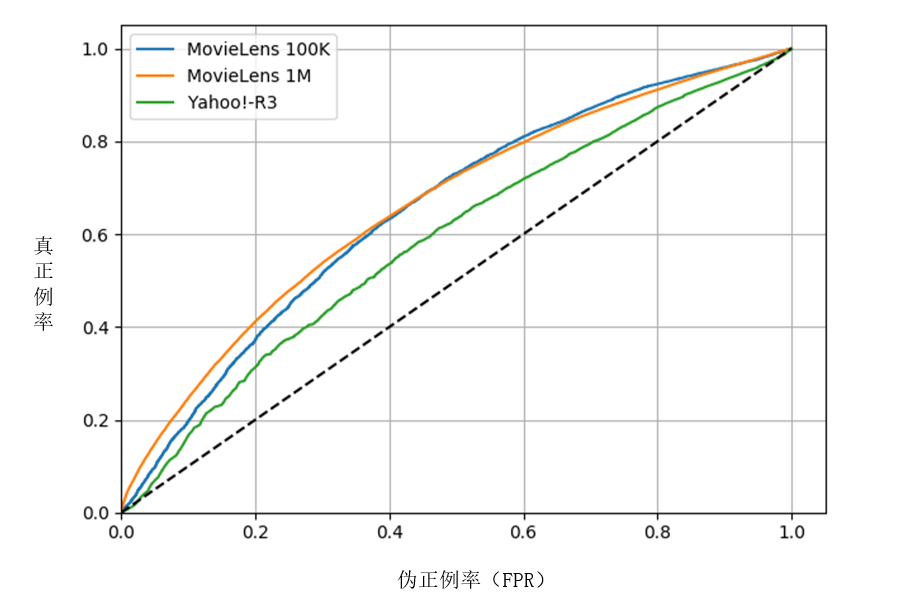
\includegraphics[width=0.7\textwidth]{2-roc.png}
	\caption{隐变量估计的ROC曲线}
	\label{Fig:ROC}
\end{figure}
\begin{table}[!]
	\centering
	\caption{隐变量的估计质量}\label{Table:ActionRecognition}
	\begin{tabular}{cccc}
		\toprule[1.2pt]
		Dataset            & MovieLens-100k &	MovieLens-1M & Yahoo!-R3 \\ \hline
		AUC               & 0.6524       &  0.6618        & 0.5885 \\
		\bottomrule[1.2pt]
	\end{tabular}
\end{table}
图~\ref{Fig:ROC}绘制了通过设置不同估计阈值的所有交互的$\hat{c}_{ui}$的ROC(接收者操作特性)曲线,并且表~\ref{Table:ActionRecognition}计算了三个数据集对应的AUC。首先承认,$\hat{c}_{ui}$的AUC性能并不是很令人满意,但它们仍然比简单猜测抛硬币要好,显著大于50\%。这意味着,BPRAC算法总体上能够为偏好较高的交互输出一个较大的$\hat{c}_{ui}$估计值,为偏好较低的交互输出一个较小的$\hat{c}_{ui}$估计值。在仅具有二元交互矩阵的有限信息下,这样的增益主要来自于后验分布的收窄,从而减小了不确定性,如公式~\eqref{Eq:Bayesian}所描述。
\par 
\textbf{个性化推荐结果性能评估}: 表~\ref{Table:Recommendation}比较了四种成对学习排序模型的推荐性能。\textsf{BPRAC}模型在所有评估指标中表现最好。 \textsf{DenoiseRec}取得了第二好的性能,表明从隐式反馈数据中去噪是必要的。然而,与\textsf{BPRAC}相比,\textsf{DenoiseRec}收敛到一个较小的AUC值,这意味着BPRAC中的参数学习比使用阈值经验确定交互是否为噪声数据更有效。此外,其余的三个对比算法都没有在隐式反馈数据中的去噪机制,每个交互都被认为是体现用户偏好的交互,这显然是不符合实际情况的。\textsf{BPRAC}的性能改进一方面表明不可信交互的存在对成对学习模型产生了不利影响;另一方面,验证了基于EM的学习模型的有效性。
\begin{table*}[!]
	\centering
	\caption{Top-k 推荐性能比较}\label{Table:Recommendation}
	\resizebox{1\textwidth}{!}{
		\begin{tabular}{llccccccccccc}
			\toprule[1.2pt]
			\multirow{2}*{\textbf{数据集}} & \multirow{2}*{\textbf{方法}}  & \multicolumn{5}{c}{Top-5} &~& \multicolumn{5}{c}{Top-10}\\ \cline{3-7} \cline{9-13}
			~&~ & Precision & Recall & F1 & NDCG & MAP&~ & Precision & Recall & F1 & NDCG & MAP \\ \cline{1-7} \cline{9-13}
			\multirow{4}*{MovieLens100K} & BPR & 0.2888 & 0.1897 & 0.1818 & 0.3401 &0.4893 &~  & 0.2379 & 0.2923 & 0.2075 & 0.3422 & 0.4663  \\
			~ & GBPR & 0.2976 & 0.1944 & 0.1872 & 0.3504 &0.4967&~ & 0.2458 & 0.3031 & 0.2147 & 0.3538 & 0.4780 \\
			~ & MPR & 0.1224 & 0.0741 & 0.0754 &0.1333& 0.2278&~ & 0.1053 & 0.1331 & 0.0935 & 0.1412 & 0.2295  \\
			~ & DenoiseRec & 0.3042 & 0.1890 & 0.1883 &0.3528&0.5122&~ & 0.2541 & 0.3027 & 0.2192 & 0.3553 & 0.4955  \\
			~& \textbf{BPRAC} & \textbf{0.3265} & \textbf{0.2158} &\textbf{0.2055}  & \textbf{0.3879} &\textbf{0.5393} &~ & \textbf{0.2665} & \textbf{0.3216} &\textbf{0.2305} & \textbf{0.3859} &\textbf{0.5127}  \\ \cline{1-7} \cline{9-13}
			
			\multirow{4}*{MovieLens1M} & BPR & 0.2940 & 0.1086 & 0.1323 & 0.3148 &0.4645&~ & 0.2570 & 0.1825 & 0.1741 & 0.3042 & 0.4517  \\
			~& GBPR & 0.3119 & 0.1265 & 0.1497 & 0.3376 &0.5004 &~ & 0.2655 & 0.2027 & 0.1874 & 0.3235 & 0.4797 \\
			~& MPR & 0.1125 & 0.0410 & 0.0494 & 0.1212 &0.2226&~ & 0.1036 & 0.0713 & 0.0681 & 0.1207 & 0.2278 \\
			~ & DenoiseRec & 0.3205 & 0.1174 & 0.1434 &0.3432&0.4996&~ &0.2737&0.1901 & 0.1831 & 0.3257 & 0.4783  \\
			~& \textbf{BPRAC} & \textbf{0.3472} & \textbf{0.1282} & \textbf{0.1572} & \textbf{0.3721} &\textbf{0.5297} &~ & \textbf{0.2992} & \textbf{0.2110} & \textbf{0.2026} & \textbf{0.3559} & \textbf{0.5044}  \\\cline{1-7} \cline{9-13}
			
			\multirow{4}*{Yahoo!-R3} & BPR & 0.0861 & 0.1007 & 0.0840 & 0.1099 & 0.1890 &~ & 0.0685 & 0.1566 & 0.0875 & 0.1284 & 0.1962  \\
			~ & GBPR & 0.1044 &0.1250 & 0.1037 & 0.1343 &0.2292&~ & 0.0817 &0.1943 & 0.1063 & 0.1576 & 0.2351  \\
			~ & MPR & 0.0694 & 0.0642 & 0.0511 & 0.0744 &0.1353&~ &0.0551 & 0.1095 & 0.0527 & 0.0875 & 0.1503  \\
			~ & DenoiseRec & 0.1058 & 0.1257 & 0.1042&0.1349&0.2247&~ & 0.0841 & 0.1993 & 0.1086 & 0.1596 & 0.2326  \\
			
			~& \textbf{BPRAC} & \textbf{0.1117} & \textbf{0.1308} & \textbf{0.1096} & \textbf{0.1448} &\textbf{0.2465}&~  & \textbf{0.0857} &\textbf{0.2034} & \textbf{0.1109} & \textbf{0.1675} & \textbf{0.2510} \\
			\bottomrule[1.2pt]
		\end{tabular}
	}
\end{table*}
\begin{figure*}[!]
	\centering
	\subfloat{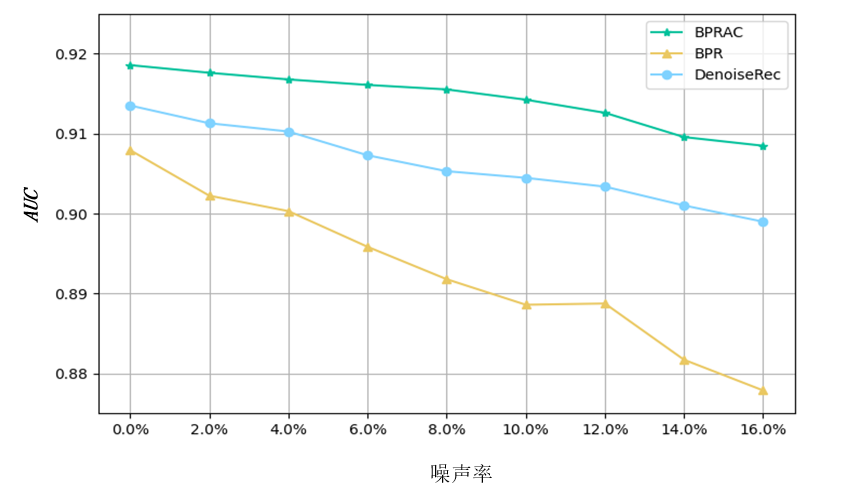
\includegraphics[width=.8\textwidth]{2-noisyratio.png}}
	\caption{不同噪声率对学习算法性能的影响}
	\label{Fig:impactd}
\end{figure*}

\textbf{对噪声数据的敏感性:}通过在训练集中随机生成噪声数据来研究\textsf{BPRAC}对噪声数据的敏感性。对比方法选择\textsf{BPR}和\textsf{DenoiseRec}。生成包含噪声的训练集时,不同的学习算法使用相同的含有噪声的训练集训练。如图~\ref{Fig:impactd}所示,噪声数据的增加导致三种学习算法的个性化推荐性能都下降,表明不可信的交互存在对学习模型产生不利影响;另一方面,由于\textsf{BPRAC}和\textsf{DenoiseRec}包含去噪机制,它们相对于\textsf{BPR}更具鲁棒性。此外,\textsf{DenoiseRec}的性能下降略多于\textsf{BPRAC},这意味着通过自适应地学习置信度,以去除噪声,比经验地通过阈值判断数据是否为噪声数据更有效。

\par
\textbf{AUC收敛性}: 图~\ref{Fig:Covergence}比较了五种算法的收敛性,度量指标为排序列表的AUC指标,这是因为优化目标函数与AUC指标是可以类比的\cite{Steffen:2009:UAI}。首先观察到,所有算法的AUC在足够的训练迭代后首先增加,然后收敛。这个试验结果也印证了引理~\ref{Lemma:ConvergenceAnalysis}的分析,如公式~\eqref{Eq:PosteriorSupremum}所示。此外注意到,与对比算法相比,本章提出的的\textsf{BPRAC}收敛到一个更高的AUC指标,代价是更慢的收敛速率从而需要更多的训练轮次,通常需要比BPR多进行2-3倍更新,这是由于引入了新的隐藏变量$c_{ui}$。这个代价是值得的,因为BPRAC提供了一种从噪声数据中学习排序的解决方案,它放宽了每个交互都表达真实偏好的强假设,取得了更好的性能。
\begin{figure}[!]
	\centering
	\subfloat{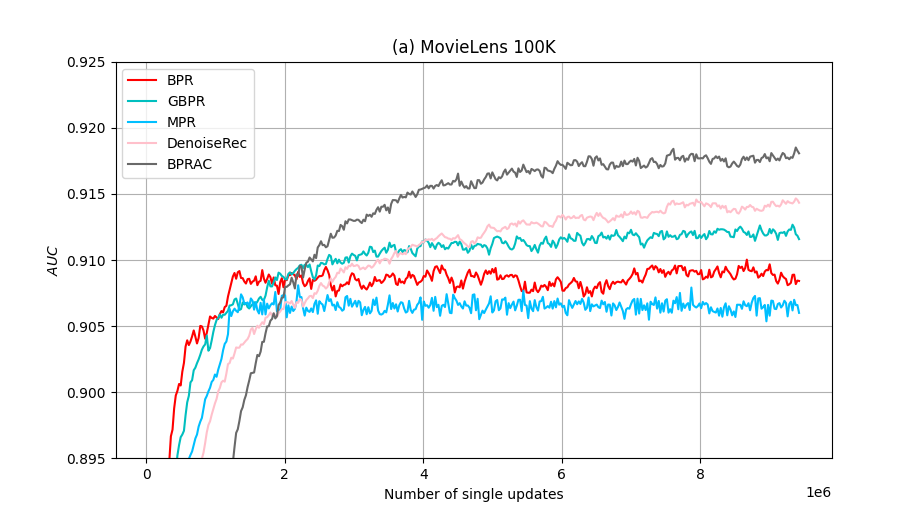
\includegraphics[width=.8\textwidth]{2-c100k.png}}\\
	\subfloat{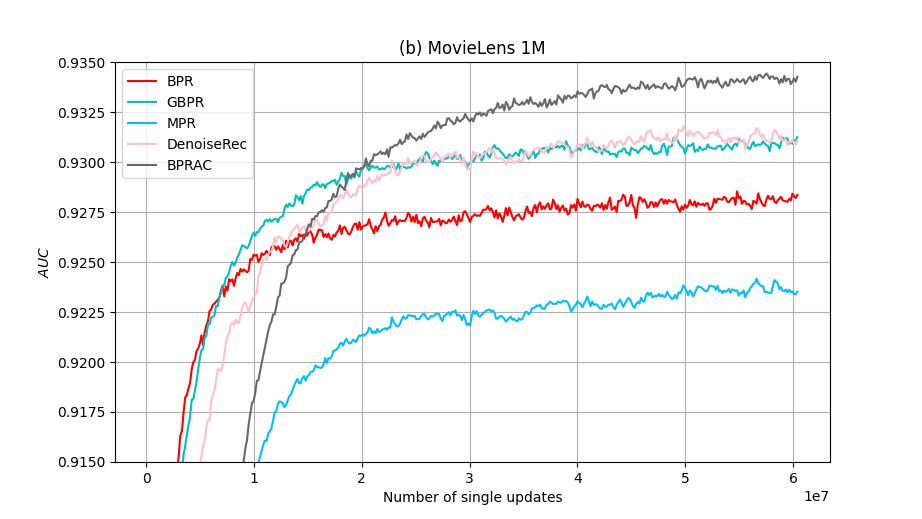
\includegraphics[width=.8\textwidth]{2-c1m.png}}\\
	\subfloat{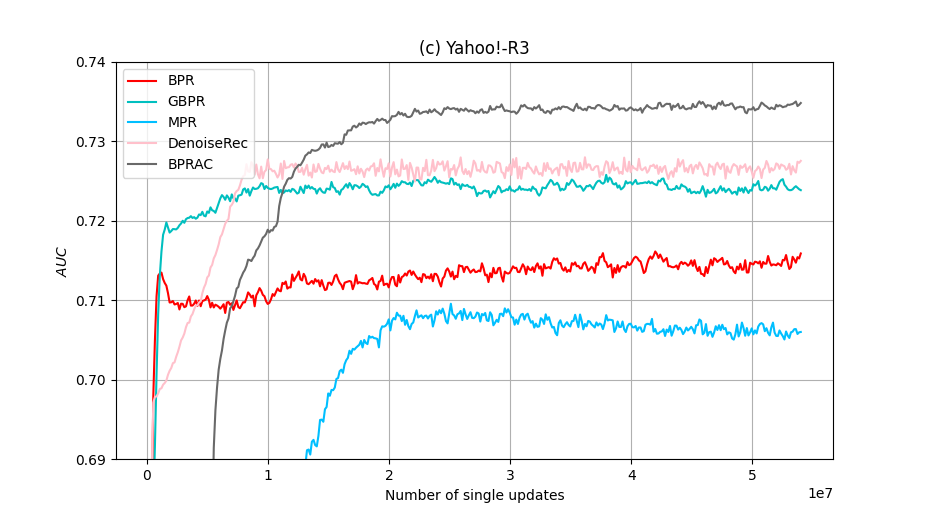
\includegraphics[width=.8\textwidth]{2-cyahoo.png}}
	\caption{不同学习算法的收敛速度比较}
	\label{Fig:Covergence}
\end{figure}

\section{本章小结}
本章聚焦于推荐系统的伪正例问题,研究了从含噪成对比较中学习排序的问题。由于隐式反馈是不完全数据,其中的伪正例构建的噪声成对比较,会对学习算法产生不利的影响。对于每个交互数据,本章引入了一个隐变量指示其可信度,并把从不完全数据中学习排序的问题形式化为一个含有隐变量的最大后验估计问题。针对这一问题,本章提出了自适应去噪的成对排序算法(BPRAC),端到端地估计隐变量并学习用户和物品表示。BPRAC算法在EM框架下求解:在E步固定模型参数估计隐变量,在M步固定隐变量学习模型参数。对真实的推荐数据集进行的实验BPRAC算法相对于其他对比方法的优越性。

值得注意的是,本章的解决方案仅限于基于矩阵分解的模型,探索如何将所提出的学习算法推广到更先进的基于神经网络的学习方法,如LightGCN~\cite{Xiangnan:2020:SIGIR}将是一个重要的问题。对于这些基于神经网络的学习方法,计算先验分布$f(\hat{x}_{ui})$是复杂的。此外,伪负例也是隐式反馈数据所面临的一个突出问题。本章的研究将为后续章节中探索更复杂模型和更一般的伪负例场景的解决方案提供启示。